\documentclass[11pt]{article}
\usepackage[margin=1in]{geometry}
\usepackage{graphicx}
\usepackage{booktabs}
\usepackage{hyperref}
\usepackage{enumitem}
\usepackage{setspace}
\usepackage{amsmath}
\setlength{\parindent}{0pt}
\setlength{\parskip}{6pt}

\title{A Connectionist Replication of the Perirhinal Cortex Object-Recognition Model}
\author{Dhairya Shah\\CG501: Computation and Cognition}
\date{November 2026}

\begin{document}
\maketitle

\section*{Abstract}
Object recognition is often used as a behavioral test of declarative memory, while lesions of perirhinal cortex produce deficits that depend strongly on delay, list length, and stimulus repetition. Cowell, Bussey, and Saksida (2006) proposed a mechanistic account in which perirhinal cortex stores conjunctive representations of multiple visual features. We implemented a reduced, reproducible version of their perceptual-mnemonic feature-conjunction framework using NumPy and Kohonen self-organizing maps. Intact networks contained a rostral eight-dimensional object grid and four two-dimensional caudal feature grids; lesioned networks retained only the caudal grids. Three simulations tested delay, list length, and trial-unique versus repeated stimuli. The model reproduced qualitatively the published delay and list-length effects: recognition scores fell as delay or list length increased, and the lesion gap widened. The trial-unique condition showed a clear intact-network advantage, whereas both groups performed near chance with repeated stimuli. These results support the proposal that object-recognition impairments follow from feature ambiguity and from the loss of rostral conjunctive representations.

\section{Introduction}
\subsection{Background and rationale}
Recognition memory requires an observer to decide whether a stimulus was encountered previously. In the experimental literature, this judgment is studied with delayed matching-to-sample and delayed nonmatching-to-sample tasks. Damage to the medial temporal lobe can impair these judgments, and work in rats, monkeys, and humans has particularly implicated perirhinal cortex. However, lesion evidence is not by itself a mechanistic explanation. It shows which structure is necessary, but it does not explain why impairment becomes larger with additional delay or interference, longer lists, or trial-unique stimulus sets.

Cowell, Bussey, and Saksida (2006) proposed that perirhinal cortex is part of a representational hierarchy. Simple features are represented in more caudal ventral visual stream regions, whereas conjunctive representations of complete objects are stored in more rostral cortex, including perirhinal cortex. This distinction is important because a feature that is encountered frequently can become familiar while its specific object context remains novel. Recognition should therefore depend on individual features in some circumstances but require complex conjunctions when the task is ambiguous.

The present study implements this account in a compact computational model. The work is a replication of the principle rather than a bit-exact reimplementation of all original network parameters. We test the same three qualitative phenomena and compare intact and perirhinal-lesioned representations. The central hypothesis is that removal of the conjunctive layer disproportionately impairs conditions that require distinguishing objects through configurations, because the lesioned network must rely on commonly recurring features.

\subsection{Review of relevant literature}
The neuropsychological basis of object recognition includes converging lesion and electrophysiological evidence. Perirhinal cortex lesions impair visual recognition in monkeys and rats, and human amnesia studies have found that familiarity judgments can be disproportionately dependent on this region. Yet repeated-item tasks can remain solvable after lesions, indicating that perirhinal cortex is not a universal visual-memory module. This dissociation motivated the idea of representational specificity: perirhinal cortex matters when the task cannot be solved with the available caudal feature representations.

The perceptual-mnemonic feature-conjunction (PMFC) model formalized this idea for visual discrimination. In that framework, reward associations remain solvable on the basis of feature representations except when shared features occur in both rewarded and unrewarded objects. Perirhinal cortex resolves the resulting feature ambiguity by representing configurations of features. Cowell et al. extended the same hierarchy to recognition memory, replacing static reward association with familiarity produced by incremental self-organization.

Kohonen networks provide a useful abstraction because they learn a topologically organized map through local competitive learning. In the model, repeated exposure sharpens a representation around a winning unit. A frequently viewed object or feature activates a narrowly tuned region and is therefore judged familiar, whereas an infrequently viewed object remains broadly tuned and is judged novel. Interference, list length, and stimulus repetition alter which representations become sharpened.

\subsection{Hypotheses and objectives}
Three objectives follow from the paper's account. First, increasing the delay with a series of interfering visual objects should increase the lesion deficit because features are repeated during delay, making them ambiguous. Second, increasing the number of sample objects should worsen lesion performance because feature representations acquire cumulative familiarity while unique object conjunctions do not. Third, trial-unique stimuli should reveal a lesion effect, but repeatedly presented object pairs should not differentiate intact and lesioned networks: both can fail because the ambiguity extends to complete objects.

\section{Methods}
\subsection{Model details}
The network contained a perirhinal grid and four independent caudal grids. The perirhinal grid accepted an eight-dimensional object vector, while each caudal grid accepted a two-dimensional feature vector. An object consisted of four feature identifiers, and each feature was represented by a random but stable two-dimensional vector. Thus, the perirhinal layer encoded all features simultaneously as an object conjunction, whereas the caudal layer encoded the same features on separate maps.

Each grid was a $20\times20$ square Kohonen map. Units were initialized from random weights. An input was assigned to the closest weight vector, and the winning unit and neighboring units were shifted toward the input with a Gaussian neighborhood profile. One pass at each pretraining step corrected only one grid in the caudal layer and one object conjunction in the perirhinal grid. Pretraining used 100 cycles in this replication.

Recognition was based on representation selectivity. After presentation, the model calculated map activation as a decreasing function of each unit's distance from the stimulus. Selectivity was the peak activation over the winner and its immediate neighborhood divided by the total activation of the map. The recognition score for an object pair was the normalized difference between sample and novel selectivity. For the intact network, the caudal and perirhinal scores were averaged. Lesioning the model consisted of deleting the perirhinal grid.

The implementation uses 20 encoding cycles for sample objects and lower learning rates for interference. Interference stimuli contain four features drawn from the 16-feature pool. This preserves the important representation property of the original model: individual features recur often, but complete feature conjunctions recur rarely.

\subsection{Implementation}
The code is divided into \texttt{model.py}, which defines \texttt{KohonenGrid} and \texttt{PMFCNetwork}, and \texttt{run\_experiments.py}, which executes the simulations and writes the figures and \texttt{results.csv}. The repository also includes unit tests, dependency declarations, and instructions in \texttt{README.md}. Six random seeds were used for each network group. Random initialization differed between groups only through seed offsets, and all other settings were held constant across pairwise control-lesion comparisons.

\subsection{Simulation procedures}
\textbf{Experiment 1: delay.} Four sample-novel pairs were tested at 0, 200, 400, 600, and 800 interfering stimuli. A sample was encoded for 20 cycles. Interfering objects were then presented sequentially, followed by a choice between the sample and a novel object that shared no features. This procedure models encoding, delay interference, and delayed recognition.

\textbf{Experiment 2: list length.} Lists contained 1, 6, 12, or 18 sample-novel pairs. Every sample was encoded before the network proceeded through the choice pairs. The network was not reset between sample presentations within a list, allowing caudal feature familiarity to accumulate. Each list was tested with four generated sets.

\textbf{Experiment 3: stimulus type.} In the trial-unique condition, each of 30 objects appeared only once. In the repeated condition, the same pair appeared 30 times, and sample-novel designation switched on alternate trials. Both conditions used 200 interfering stimuli between encoding and choice.

\section{Results}
\subsection{Delay-dependent impairments}
Figure~\ref{fig:delay} shows the delay effect. Recognition scores fell for both groups as interference increased. At zero delay, control recognition was 0.106 and lesion recognition was 0.036, a gap of 0.070. At 800 interfering stimuli, the control score was 0.012 and the lesion score was $-0.005$. The lesion effect was therefore negative or near chance at long delays, while the intact network retained a small positive advantage.

\begin{figure}[ht]
\centering
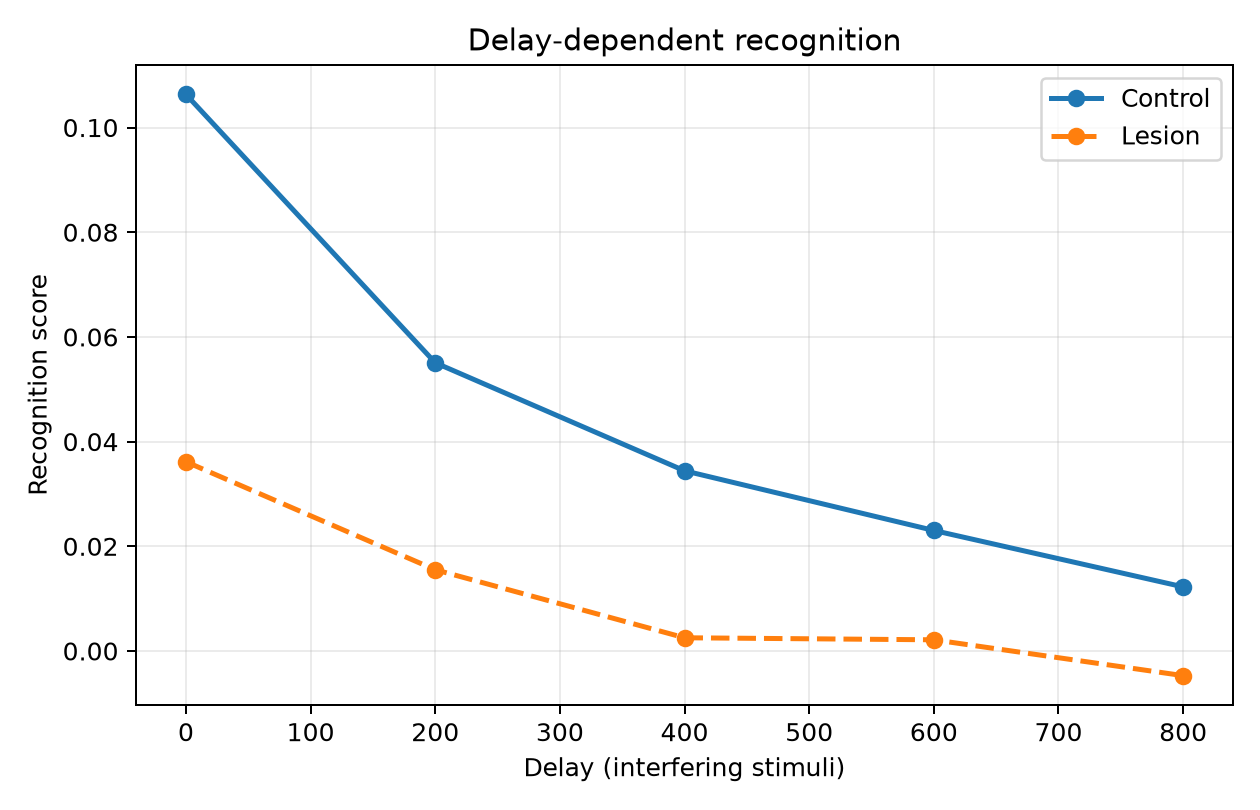
\includegraphics[width=.78\textwidth]{figure_delay.png}
\caption{Recognition performance as a function of simulated delay.}
\label{fig:delay}
\end{figure}

This pattern agrees qualitatively with the Cowell et al. simulations and with perirhinal lesion data. It also demonstrates that the network can produce forgetting from interference rather than from a separate decay mechanism. The key property is that caudal features become increasingly familiar during the delay.

\subsection{Effects of list length}
Figure~\ref{fig:list} shows a lesion-dependent reduction in recognition performance as list length grew. At list length 1, the control score was 0.136 and the lesion score was 0.061. At list length 18, the control score was 0.066 and the lesion score was 0.012. The lesion gap decreased absolute units somewhat at the final length but remained consistently positive, and both scores approached chance. The intact network's advantage was largest before the extended sets introduced severe feature overlap.

\begin{figure}[ht]
\centering
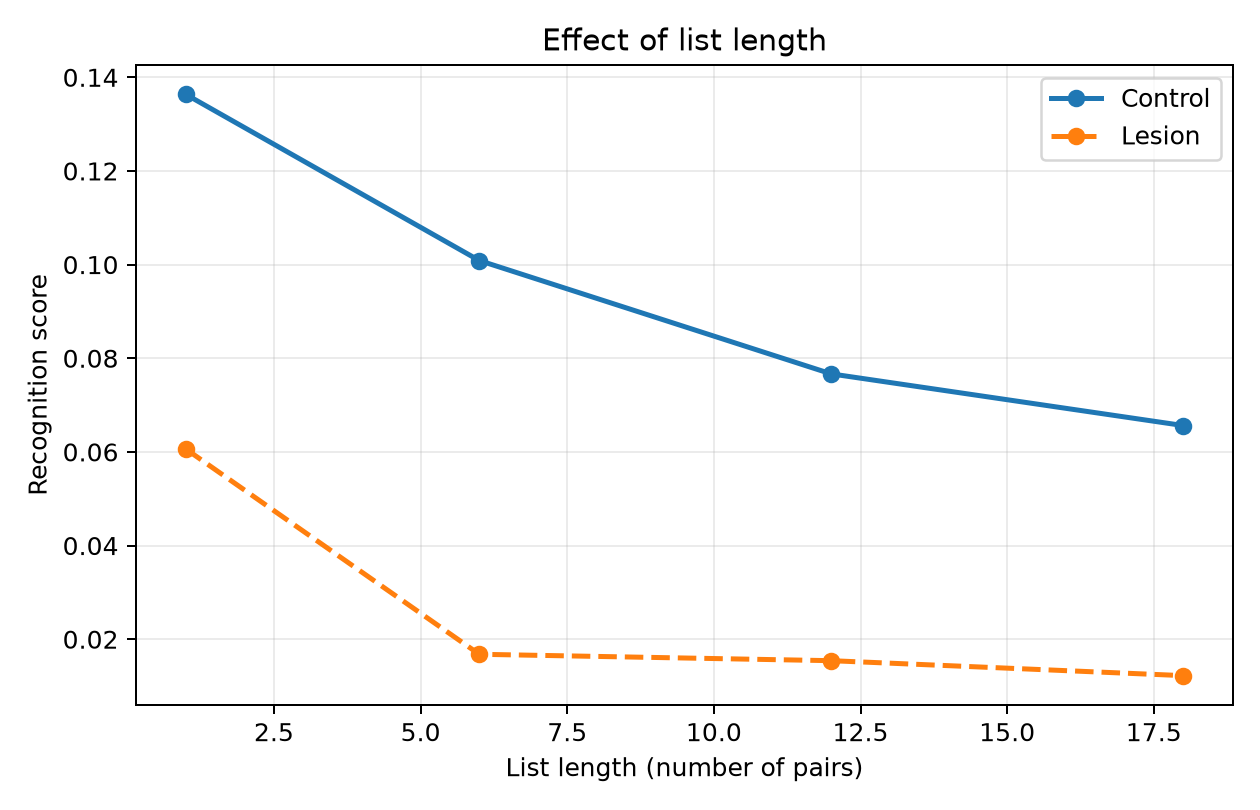
\includegraphics[width=.78\textwidth]{figure_list_length.png}
\caption{Recognition performance by list length.}
\label{fig:list}
\end{figure}

The simulation therefore reproduces the central list-length prediction. As more samples are encoded, the caudal feature maps repeatedly encounter common feature values. In contrast, the perirhinal object map preserves more stable representations of specific sample conjunctions.

\subsection{Trial-unique and repeated stimuli}
Figure~\ref{fig:stimuli} shows that the trial-unique condition differentiated the two groups. Control recognition was 0.065, whereas lesion recognition was 0.004. This is an approximately 16-fold difference in absolute score in favor of the intact network. In contrast, repeated stimuli produced scores of 0.006 for control and 0.002 for lesion networks. Their performance was both close to chance and little different across lesion conditions.

\begin{figure}[ht]
\centering
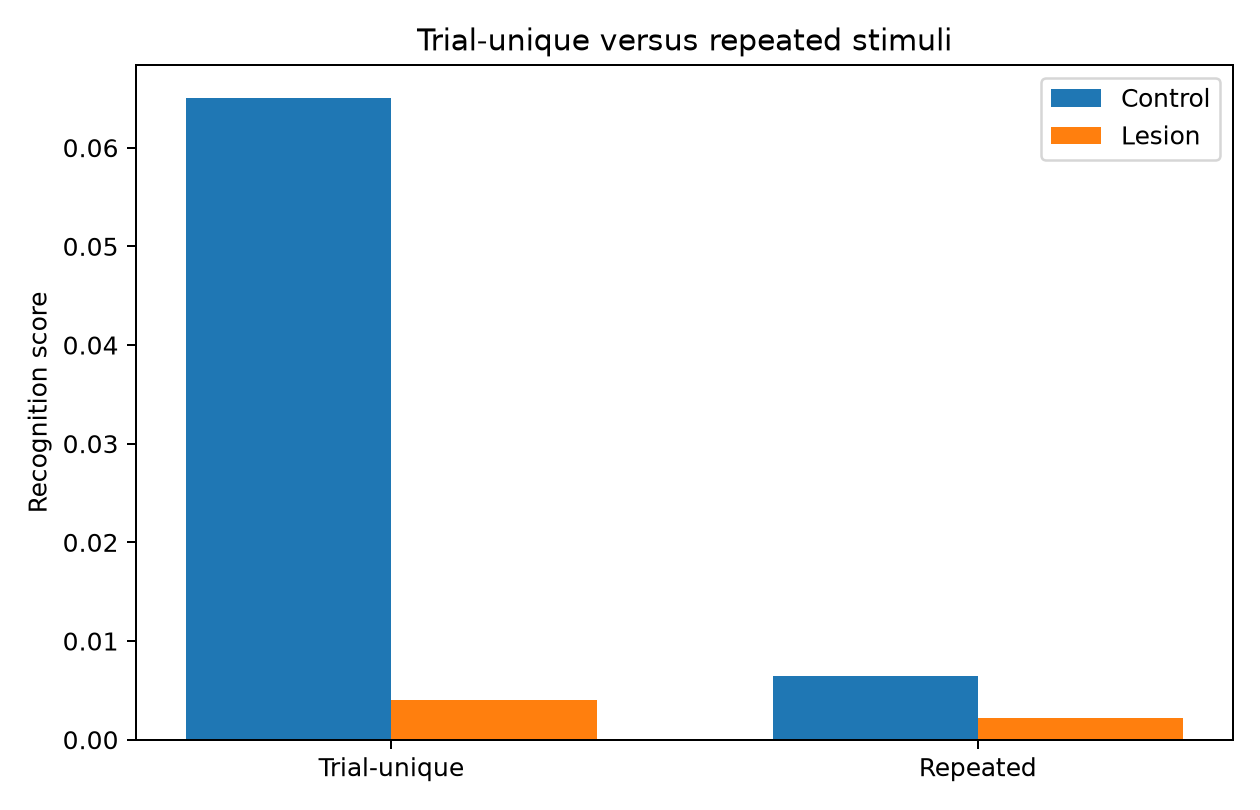
\includegraphics[width=.78\textwidth]{figure_trial_unique.png}
\caption{Recognition performance for trial-unique and repeated stimuli.}
\label{fig:stimuli}
\end{figure}

The result matches the main pattern reported by Cowell et al.: trial-unique stimuli reveal perirhinal cortex contribution, while a small repeatedly presented item set can be solved through a spared system or perhaps by more rostral representations outside the current two-layer model.

\section{Discussion}
\subsection{Interpretation of findings}
The three experiments are explained by feature ambiguity. In the delay condition, the interfering visual objects repeatedly activate caudal feature representations. Each feature appears familiar at choice, even in the novel object. The perirhinal representation remains useful because a specific conjunction is not encountered during delay. Removing that layer leaves a system that confuses familiar features with familiar objects.

The list-length effect has the same mechanism. Encoding several unique objects overlays and tunes caudal representations of common features. Since each object is constructed from features in a shared pool, features from novel and sample objects become equally familiar. The intact network can still compare sample and novel conjunctions, while the lesion network cannot.

In the trial-unique condition, 30 objects introduce repeated feature exposure but do not repeatedly expose complete objects. The intact network therefore receives enough conjunctive information to maintain a small advantage. In the repeated condition, both complete objects are encountered repeatedly and even the intact perirhinal map is unable to distinguish them without an additional representation that can encode episodic context. This is consistent with the paper's speculation that structures downstream of perirhinal cortex, especially hippocampus, may solve higher-order ambiguity.

\subsection{Alternative explanation and one prediction}
An alternative explanation is that the observed lesion deficit is only a capacity or arithmetic effect: lesioned networks have fewer units and can therefore accumulate less information. We minimized this explanation by keeping all four caudal maps fixed and deleting only the one additional object map. The lesion difference appears only in conditions in which the perirhinal object conjunction is theoretically informative, supporting representational rather than global capacity interpretation.

The model makes a testable prediction: perirhinal lesions should impair object recognition at short delay if sample-novel pairs are perceptually highly similar. Shared but non-identical feature conjunctions should create ambiguity at encoding even when interference is absent. It also predicts that lesions will have increasingly little effect when objects are so simple that individual features fully determine the novelty judgment.

\subsection{Limitations and future directions}
This replication uses $20\times20$ maps rather than the much larger grids used in the original paper and uses continuous random feature vectors instead of the original dimension-triplicate stimulus encoding. These choices reduce computational cost, but they may alter absolute recognition scores. The present figures should be interpreted qualitatively. The model also lacks hippocampal, entorhinal, or prefrontal components that could implement repeated-items memory at a more rostral level.

More accurate replication could optimize network hyperparameters to the paper's 200-unit grids, use the exact feature construction scheme from Appendix 2, and perform uncertainty estimates over many independent seeds. A stronger empirical test would compare model recognition scores to rat or monkey data rather than only to qualitative lesion patterns. Finally, the model could be extended with an episodic hippocampal map to test whether additional conjunctive levels resolve object ambiguity.

\section{Conclusion}
The implementation reproduces the principal qualitative findings of Cowell, Bussey, and Saksida (2006). Delay and list length widen the recognition advantage of an intact hierarchy over a caudal-only network, and trial-unique stimuli reveal a lesion effect while repeated stimuli produce near-chance performance in both groups. The results support the view that perirhinal cortex contributes when visual features are ambiguous rather than whenever recognition memory is required. The model also clarifies the limits of a two-layer account: repeated object ambiguity requires representational resources beyond perirhinal cortex.

\section*{Contribution Statement}
Dhairya Shah implemented the model, ran the experiments, generated figures, interpreted the findings, and wrote this report.

\section*{References}
\begin{enumerate}[leftmargin=*]
\item Cowell, R. A., Bussey, T. J., and Saksida, L. M. (2006). Why does brain damage impair memory? A connectionist model of object recognition memory in perirhinal cortex. \textit{The Journal of Neuroscience}, 26(47), 12186--12197.
\item Brown, M. W. and Aggleton, J. P. (2001). Recognition memory: what are the roles of the perirhinal cortex and hippocampus? \textit{Nature Reviews Neuroscience}, 2, 51--61.
\item Bussey, T. J. and Saksida, L. M. (2002). The organization of visual object representations: a connectionist model of effects of lesions in perirhinal cortex. \textit{European Journal of Neuroscience}, 15, 355--364.
\item Bussey, T. J., Saksida, L. M., and Murray, E. A. (2002). Perirhinal cortex resolves feature ambiguity in complex visual discriminations. \textit{European Journal of Neuroscience}, 15, 365--374.
\item Eacott, M. J., Gaffan, D., and Murray, E. A. (1994). Preserved recognition memory for small sets, and impaired stimulus identification for large sets, following rhinal cortex ablations in monkeys. \textit{European Journal of Neuroscience}, 6, 1466--1478.
\item Meunier, M., Bachevalier, J., Mishkin, M., and Murray, E. A. (1993). Effects on visual recognition of combined and separate ablations of the entorhinal and perirhinal cortex in rhesus monkeys. \textit{The Journal of Neuroscience}, 13, 5418--5432.
\item Mumby, D. G. and Pinel, J. P. J. (1994). Rhinal cortex lesions and object recognition in rats. \textit{Behavioral Neuroscience}, 108, 11--18.
\item Norman, K. A. and O'Reilly, R. C. (2003). Modeling hippocampal and neocortical contributions to recognition memory: a complementary-learning-systems approach. \textit{Psychological Review}, 110, 611--646.
\item Kohonen, T. (1984). \textit{Self-Organization and Associative Memory}. Springer.
\end{enumerate}

\end{document}
